\documentclass{resume} % Use the custom resume.cls style

\usepackage[left=0.75in,top=0.6in,right=0.75in,bottom=0.6in]{geometry} % Document margins
\usepackage{graphicx}
\graphicspath{{images/}}
\name{Aniket Patel} % Your name
\address{G-7/10,Janta Housing, Jesal Park, Bhayandar(East), Thane-401105} % Your address
\address{+918655528032 \\ aniket10051994@gmail.com} % Your phone number and email
\begin{document}
	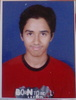
\includegraphics{aniket-002}
	
\begin{rSection}{Career Objective}
		To give full dedication and commitment to the assigned work and produce the best results out of it
\end{rSection}
	
\begin{rSection}{Education}
	\begin{center}
		\begin{tabular}{||c|c|c|c||}
			\hline\hline
			\bf Examination & \bf Institute & \bf year & \bf Performance \\
			\hline\hline 
			3rd Year B.Tech & Veermata Jijabai Technological Institute & May, 2015 & 8.3 CGPA \\
			\hline
			H.S.C & D.G. Ruparel College & 2012 & 86.33\% \\
			\hline
			S.S.C & St.Francis High School & 2010 & 93.64\% \\
			\hline\hline
			
			
		\end{tabular}
	\end{center}
	
\end{rSection}

\begin{rSection}{Projects}
	
	\begin{enumerate}
		
		\item \begin{rSubsection}{Home Automation}{May, 2013}{Mechanical \& Electronics}{VJTI, Eklavya}
			\item Automating a house and controlling the basic devices like lights, fans, doors, curtains,etc with the help of an android system phone via a bluetooth.
		\end{rSubsection}
		
		\item \begin{rSubsection}{Voice Controlled Crane(VCC)}{December, 2013}{Mechanical \& Electroncs}{VJTI, Technovanza}
			\item A crane that could be voice controlled where the commands are given on the microphone of android phone and the commands like pick, go, stop, up, down,etc are executed by the crane.
			\item The crane could be controlled from a Remote distance.
		\end{rSubsection}
	\end{enumerate}
\end{rSection}

\begin{rSection}{Training and Internship}
	\begin{itemize}
		\item \begin{rSubsection}{Wall-E(Workshop)}{December, 2012}{Coding \& Electroncs}{VJTI, SRA}
			\item Participated in ROBO-based workshop and learnt the basics of line following robot
		\end{rSubsection}
		\item Never did any internship
	\end{itemize}
\end{rSection}

\begin{rSection}{Research Publication}
	\begin{enumerate}
		\item Read a research paper on "Vehicle Crash Test using Haar Wavelets" as a part of an academic activity.
		\item No research paper publication yet
	\end{enumerate}
\end{rSection}

\newpage
\begin{rSection}{Technical Skills}
	\begin{itemize}
		\item C++, C, Embedded C
		\item Coding and Debugging
		\item Matlab
		\item Eclipse and Android Studio
		\item Robotics 
	\end{itemize}
\end{rSection}
\begin{rSection}{Soft Skills}
	\begin{enumerate}
		\item Good communication skills
		\item Good presentation skills
	\end{enumerate}
\end{rSection}
\begin{rSection}{Extra-Curricular Activities}
	\begin{itemize}
		\item \begin{rSubsection}{Contraption}{December, 2014}{Mechanical \& Electroncs}{VJTI, Technovanza}
			\item Event head of Contraption- A mechanical and electronics project and was exhibited at Technovanza Festival
		\end{rSubsection}
		\item \begin{rSubsection}{Cargo Sorting}{March, 2015}{Mechanical, Coding \& Electroncis}{IIT Bombay, E-Yantra}
			\item Participated in a National Level Robotics Challenge organised by IIT Bombay and grabbed 1st Place among 52 teams.
		\end{rSubsection}
		\item Learning Data Structures and Algorithm
		\item Web Designing and Android App development
		\item Networking
	\end{itemize}
\end{rSection}
\begin{rSection}{Co-Curricular activities}
	\begin{enumerate}
		\item Digital Signal Processing on Matlab
		\item Speech Processing on Matlab
		\item Learning Machine Learning Algorithms
	\end{enumerate}
\end{rSection}

\begin{rSection}{Personal Information}
	\item \textbf{Father’s Name:} Deepak Patel
	\item \textbf{Mother’s Name: } Punita Patel
	\item \textbf{Sex:} Male
	\item \textbf{Date of Birth:} 10th May,1994 
	\item \textbf{Nationality: } Hindu
	\item \textbf{Marital Status:}	Single
\end{rSection}

\newpage
\begin{rSection}{Reference}
	Prof. Aakanksha Chauhan,
	\newline
	VJTI, Matunga, Mumbai,
	\newline
	Email Id: akanksha22.chauhan@gmail.com
	
\end{rSection}
\begin{rSection}{Declaration}
	I hereby declare that the above written particulars are true to the best of my knowledge and belief.
\end{rSection}

\begin{rSection}
	\bf Date 23rd May, 2015
\end{rSection}


\end{document}